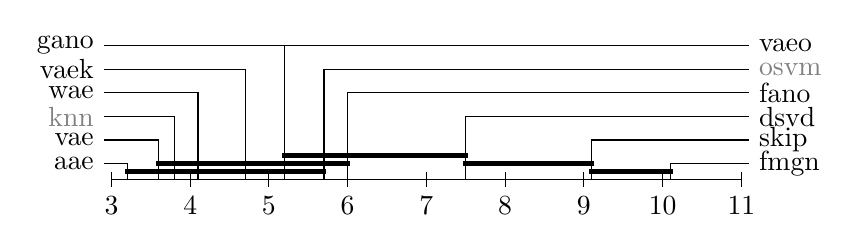
\begin{tikzpicture}[scale=1.0] 
  \draw (3.0,0) -- (11.0,0); 
  \foreach \x in {3,...,11} \draw (\x,0.10) -- (\x,-0.10) node[anchor=north]{$\x$}; 
  \draw (3.2,0) -- (3.2,0.19999999999999998) -- (2.9, 0.19999999999999998) node[anchor=east] {aae}; 
  \draw (3.6,0) -- (3.6,0.5) -- (2.9, 0.5) node[anchor=east] {vae}; 
  \draw (3.8,0) -- (3.8,0.7999999999999999) -- (2.9, 0.7999999999999999) node[anchor=east] {\textcolor{gray}{knn}}; 
  \draw (4.1,0) -- (4.1,1.0999999999999999) -- (2.9, 1.0999999999999999) node[anchor=east] {wae}; 
  \draw (4.7,0) -- (4.7,1.4) -- (2.9, 1.4) node[anchor=east] {vaek}; 
  \draw (5.2,0) -- (5.2,1.6999999999999997) -- (2.9, 1.6999999999999997) node[anchor=east] {gano}; 
  \draw (5.2,0) -- (5.2,1.7) -- (11.1, 1.7) node[anchor=west] {vaeo}; 
  \draw (5.7,0) -- (5.7,1.4) -- (11.1, 1.4) node[anchor=west] {\textcolor{gray}{osvm}}; 
  \draw (6.0,0) -- (6.0,1.0999999999999999) -- (11.1, 1.0999999999999999) node[anchor=west] {fano}; 
  \draw (7.5,0) -- (7.5,0.8) -- (11.1, 0.8) node[anchor=west] {dsvd}; 
  \draw (9.1,0) -- (9.1,0.5) -- (11.1, 0.5) node[anchor=west] {skip}; 
  \draw (10.1,0) -- (10.1,0.2) -- (11.1, 0.2) node[anchor=west] {fmgn}; 
  \draw[line width=0.06cm,color=black,draw opacity=1.0] (3.1700000000000004,0.1) -- (5.73,0.1); 
  \draw[line width=0.06cm,color=black,draw opacity=1.0] (3.5700000000000003,0.2) -- (6.03,0.2); 
  \draw[line width=0.06cm,color=black,draw opacity=1.0] (5.17,0.30000000000000004) -- (7.53,0.30000000000000004); 
  \draw[line width=0.06cm,color=black,draw opacity=1.0] (7.47,0.2) -- (9.129999999999999,0.2); 
  \draw[line width=0.06cm,color=black,draw opacity=1.0] (9.07,0.1) -- (10.129999999999999,0.1); 
 \end{tikzpicture} 
